\documentclass{article}

\usepackage[top=0.9in, bottom=1in, left=1.5in, right=1.5in]{geometry}
\usepackage[utf8]{inputenc}
\usepackage[icelandic]{babel}
\usepackage[T1]{fontenc}
\usepackage[sc]{mathpazo} % Palatino font

\usepackage[parfill]{parskip}
\usepackage{booktabs,tabularx}
\usepackage{multirow}
\usepackage{graphicx}
\usepackage{gensymb}
\usepackage{amsmath}
\usepackage{minted} %Minted and configuration

\usepackage[pdftex,bookmarks=true,colorlinks=true,pdfauthor={Eirikur Ernir Thorsteinsson},linkcolor=blue,urlcolor=blue]{hyperref}

\usemintedstyle{default}
\renewcommand{\theFancyVerbLine}{\sffamily \arabic{FancyVerbLine}}

\date{Vorönn 2016}
\author{}

\hyphenpenalty=5000

\setcounter{secnumdepth}{-1} 
\pagenumbering{gobble}

\title{FOR3R3U Skilaverkefni 5 - net}

\begin{document}

\maketitle
\section{Verkefni}
Skilið inn eftirfarandi dæmum.

\subsection{Net}

Skilgreinið netið á eftirfarandi mynd í Python:

\begin{center}
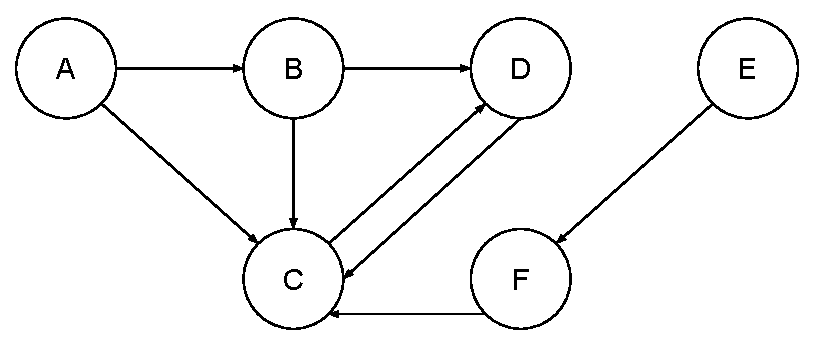
\includegraphics[width=0.8\textwidth]{Pics/Net}
\end{center}

Þetta er mögulegt að gera með hlutbundinni forritun, en einfaldast er að nota dictionary og lista.

\subsection{Breiðleit}

Skrifið breiðleitarreiknirit (e. \emph{breadth-first-search}) sem virkar á netið.

\subsection{Djúpleit}

Skrifið djúpleitarreiknirit (e. \emph{depth-first-search}) sem virkar á netið.


\end{document}